% Decorated G2-trees of orbit 21 (Coarsest G2 Grassmannian cell 155: rays 7,12,40): the star with an apple on its pendant edge to taxon 1, the ray 7 with an apple at A and the cell with an apple on AB, generated by julia/to_tex/decorated_trees_figure.jl
% The star with an apple on its pendant edge to taxon 1; ray 7 with an apple at its inner vertex A (vertex 8 of its tree); the cell with an apple on its edge AB (vertices 10 and 11 of its tree).
% Letters of the inner vertices of the rays, in the order of the rays 7,12,40:
%   A: the side {3,4} of its edges
%   B: the side {1,2,5,6,7} of its edges
%   C: the side {1,5} of its edges
%   D: the side {2,3,4,6,7} of its edges
%   E: the side {1,3,4,5,7} of its edges
%   F: the side {2,6} of its edges
\begingroup
\definecolor{g2RayLabel}{HTML}{000000}
\definecolor{g2CellLabel}{HTML}{000000}
\definecolor{g2AppleBody}{HTML}{7CB342}
\definecolor{g2AppleDark}{HTML}{33691E}
\definecolor{g2AppleLeaf}{HTML}{1B5E20}
\definecolor{g2AppleStem}{HTML}{5D4037}
\tikzset{
g2square name/.style={text=g2RayLabel,inner sep=0pt,font=\boldmath},
g2square cell name/.style={g2square name,text=g2CellLabel},
pics/g2apple/.style={code={
  \path[fill=g2AppleBody]
    (0mm,-1.95mm)..controls(.6mm,-1.25mm)and(2.3mm,-1.3mm)..(2.3mm,-3mm)
    ..controls(2.3mm,-4.7mm)and(1.3mm,-5.8mm)..(.6mm,-5.7mm)
    ..controls(.3mm,-5.65mm)and(-.3mm,-5.65mm)..(-.6mm,-5.7mm)
    ..controls(-1.3mm,-5.8mm)and(-2.3mm,-4.7mm)..(-2.3mm,-3mm)
    ..controls(-2.3mm,-1.3mm)and(-.6mm,-1.25mm)..(0mm,-1.95mm)--cycle;
  \draw[g2AppleStem,line width=.6pt,line cap=round]
    (0mm,0mm)..controls(.08mm,-.8mm)..(-.05mm,-2mm);
  \path[fill=g2AppleLeaf]
    (.03mm,-1.15mm)..controls(.45mm,-.5mm)and(1.25mm,-.45mm)..(1.75mm,-.85mm)
    ..controls(1.25mm,-1.35mm)and(.55mm,-1.5mm)..(.03mm,-1.15mm)--cycle;
}},
}
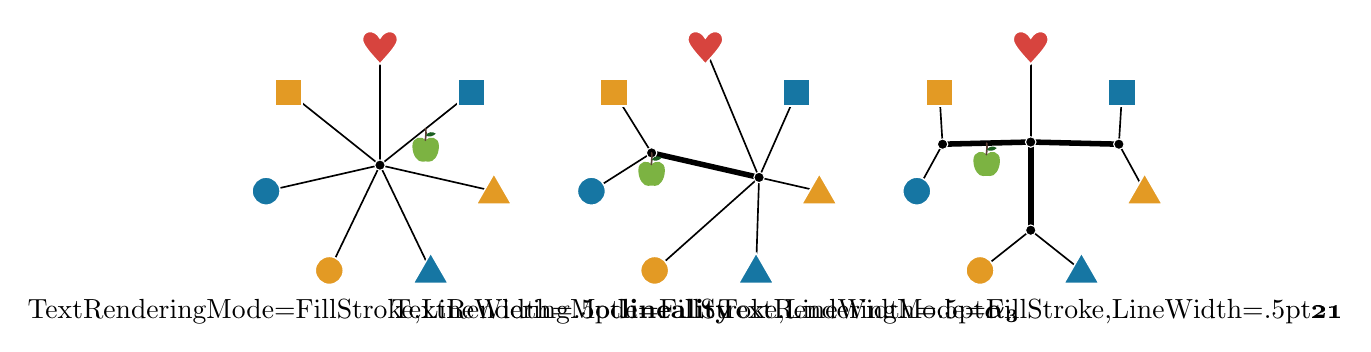
\begin{tikzpicture}[x=1cm,y=1cm,baseline=(current bounding box.center)]
\begin{scope}[shift={(-6.1984,0.0)}]
\begingroup
\definecolor{g2TaxonBlue}{HTML}{1676A3}
\definecolor{g2TaxonYellow}{HTML}{E39A24}
\definecolor{g2HeartRed}{HTML}{D7443E}
\tikzset{
  g2tree pendant/.style={draw=black,line width=.6pt,line cap=round},
  g2tree internal/.style={draw=black,line width=2pt,line cap=round},
  g2tree vertex/.style={circle,fill=black,draw=white,line width=.4pt,inner sep=0pt,minimum size=3.8pt},
  g2tree dark/.style={fill=g2TaxonBlue,draw=white,line width=.55pt,text=white,inner sep=0pt},
  g2tree light/.style={fill=g2TaxonYellow,draw=white,line width=.55pt,text=white,inner sep=0pt},
  g2tree weight/.style={circle,fill=white,draw=none,text=black,inner sep=.15pt,minimum size=8.5pt},
  g2tree aligned pendant/.style={fill=white,text=black,inner sep=.7pt,sloped,above=1pt,font={\sffamily\fontsize{7.5}{8}\selectfont}},
  g2tree aligned internal/.style={fill=white,text=black,inner sep=1pt,sloped,above=1pt,font={\sffamily\fontsize{7.5}{8}\selectfont\bfseries}},
}
\coordinate (v1) at (1.16024,0.92526);
\coordinate (v2) at (0.64388,-1.33704);
\coordinate (v3) at (-1.44679,-0.33022);
\coordinate (v4) at (-1.16024,0.92526);
\coordinate (v5) at (1.44679,-0.33022);
\coordinate (v6) at (-0.64388,-1.33704);
\coordinate (v7) at (0.00000,1.48400);
\coordinate (v8) at (0.00000,0.00000);
\draw[g2tree pendant] (v1)--(v8);
\draw[g2tree pendant] (v2)--(v8);
\draw[g2tree pendant] (v3)--(v8);
\draw[g2tree pendant] (v4)--(v8);
\draw[g2tree pendant] (v5)--(v8);
\draw[g2tree pendant] (v6)--(v8);
\draw[g2tree pendant] (v7)--(v8);
\node[g2tree vertex] at (v8) {};
\node[g2tree dark,rectangle,minimum size=3.4155000000000006mm,font={\sffamily\fontsize{6.6}{6.6}\selectfont\bfseries}] at (v1) {};
\begin{scope}[shift={(v2)},scale=0.7425000000000002,transform shape]
\path[fill=g2TaxonBlue,draw=white,line width=.55pt,line join=round] (0mm,3.0mm)--(-3.0mm,-2.2mm)--(3.0mm,-2.2mm)--cycle;
\end{scope}
\node[g2tree dark,circle,minimum size=3.5640000000000005mm,font={\sffamily\fontsize{6.6}{6.6}\selectfont\bfseries}] at (v3) {};
\node[g2tree light,rectangle,minimum size=3.4155000000000006mm,font={\sffamily\fontsize{6.6}{6.6}\selectfont\bfseries}] at (v4) {};
\begin{scope}[shift={(v5)},scale=0.7425000000000002,transform shape]
\path[fill=g2TaxonYellow,draw=white,line width=.55pt,line join=round] (0mm,3.0mm)--(-3.0mm,-2.2mm)--(3.0mm,-2.2mm)--cycle;
\end{scope}
\node[g2tree light,circle,minimum size=3.5640000000000005mm,font={\sffamily\fontsize{6.6}{6.6}\selectfont\bfseries}] at (v6) {};
\begin{scope}[shift={(v7)},scale=0.7425000000000002,transform shape]
\path[fill=g2HeartRed,draw=white,line width=.55pt]
  (0mm,-2.7mm)..controls(-.45mm,-2.1mm)and(-3.0mm,.35mm)..(-3.0mm,1.45mm)
  ..controls(-3.0mm,3.2mm)and(-.9mm,3.4mm)..(0mm,1.75mm)
  ..controls(.9mm,3.4mm)and(3.0mm,3.2mm)..(3.0mm,1.45mm)
  ..controls(3.0mm,.35mm)and(.45mm,-2.1mm)..(0mm,-2.7mm)--cycle;
\end{scope}
\endgroup
\pic[rotate=0,scale=0.7333] at (0.5801,0.4626) {g2apple};
\end{scope}
\node[anchor=north,g2square name] at (-6.1984,-1.6992) {\textpdfrender{TextRenderingMode=FillStroke,LineWidth=.5pt}{\bfseries\boldmath lineality}};
\begin{scope}[shift={(-2.0662,0.0)}]
\begingroup
\definecolor{g2TaxonBlue}{HTML}{1676A3}
\definecolor{g2TaxonYellow}{HTML}{E39A24}
\definecolor{g2HeartRed}{HTML}{D7443E}
\tikzset{
  g2tree pendant/.style={draw=black,line width=.6pt,line cap=round},
  g2tree internal/.style={draw=black,line width=2pt,line cap=round},
  g2tree vertex/.style={circle,fill=black,draw=white,line width=.4pt,inner sep=0pt,minimum size=3.8pt},
  g2tree dark/.style={fill=g2TaxonBlue,draw=white,line width=.55pt,text=white,inner sep=0pt},
  g2tree light/.style={fill=g2TaxonYellow,draw=white,line width=.55pt,text=white,inner sep=0pt},
  g2tree weight/.style={circle,fill=white,draw=none,text=black,inner sep=.15pt,minimum size=8.5pt},
  g2tree aligned pendant/.style={fill=white,text=black,inner sep=.7pt,sloped,above=1pt,font={\sffamily\fontsize{7.5}{8}\selectfont}},
  g2tree aligned internal/.style={fill=white,text=black,inner sep=1pt,sloped,above=1pt,font={\sffamily\fontsize{7.5}{8}\selectfont\bfseries}},
}
\coordinate (v1) at (1.16024,0.92526);
\coordinate (v2) at (0.64388,-1.33704);
\coordinate (v3) at (-1.44679,-0.33022);
\coordinate (v4) at (-1.16024,0.92526);
\coordinate (v5) at (1.44679,-0.33022);
\coordinate (v6) at (-0.64388,-1.33704);
\coordinate (v7) at (0.00000,1.48400);
\coordinate (v8) at (-0.68245,0.15576);
\coordinate (v9) at (0.68245,-0.15576);
\draw[g2tree internal] (v8)--(v9);
\draw[g2tree pendant] (v1)--(v9);
\draw[g2tree pendant] (v2)--(v9);
\draw[g2tree pendant] (v3)--(v8);
\draw[g2tree pendant] (v4)--(v8);
\draw[g2tree pendant] (v5)--(v9);
\draw[g2tree pendant] (v6)--(v9);
\draw[g2tree pendant] (v7)--(v9);
\node[g2tree vertex] at (v8) {};
\node[g2tree vertex] at (v9) {};
\node[g2tree dark,rectangle,minimum size=3.4155000000000006mm,font={\sffamily\fontsize{6.6}{6.6}\selectfont\bfseries}] at (v1) {};
\begin{scope}[shift={(v2)},scale=0.7425000000000002,transform shape]
\path[fill=g2TaxonBlue,draw=white,line width=.55pt,line join=round] (0mm,3.0mm)--(-3.0mm,-2.2mm)--(3.0mm,-2.2mm)--cycle;
\end{scope}
\node[g2tree dark,circle,minimum size=3.5640000000000005mm,font={\sffamily\fontsize{6.6}{6.6}\selectfont\bfseries}] at (v3) {};
\node[g2tree light,rectangle,minimum size=3.4155000000000006mm,font={\sffamily\fontsize{6.6}{6.6}\selectfont\bfseries}] at (v4) {};
\begin{scope}[shift={(v5)},scale=0.7425000000000002,transform shape]
\path[fill=g2TaxonYellow,draw=white,line width=.55pt,line join=round] (0mm,3.0mm)--(-3.0mm,-2.2mm)--(3.0mm,-2.2mm)--cycle;
\end{scope}
\node[g2tree light,circle,minimum size=3.5640000000000005mm,font={\sffamily\fontsize{6.6}{6.6}\selectfont\bfseries}] at (v6) {};
\begin{scope}[shift={(v7)},scale=0.7425000000000002,transform shape]
\path[fill=g2HeartRed,draw=white,line width=.55pt]
  (0mm,-2.7mm)..controls(-.45mm,-2.1mm)and(-3.0mm,.35mm)..(-3.0mm,1.45mm)
  ..controls(-3.0mm,3.2mm)and(-.9mm,3.4mm)..(0mm,1.75mm)
  ..controls(.9mm,3.4mm)and(3.0mm,3.2mm)..(3.0mm,1.45mm)
  ..controls(3.0mm,.35mm)and(.45mm,-2.1mm)..(0mm,-2.7mm)--cycle;
\end{scope}
\endgroup
\pic[rotate=0,scale=0.7333] at (-0.6824,0.1558) {g2apple};
\end{scope}
\node[anchor=north,g2square name] at (-2.0662,-1.6992) {\textpdfrender{TextRenderingMode=FillStroke,LineWidth=.5pt}{\bfseries\boldmath \(\alpha_3\)}};
\begin{scope}[shift={(2.0662,0.0)}]
\begingroup
\definecolor{g2TaxonBlue}{HTML}{1676A3}
\definecolor{g2TaxonYellow}{HTML}{E39A24}
\definecolor{g2HeartRed}{HTML}{D7443E}
\tikzset{
  g2tree pendant/.style={draw=black,line width=.6pt,line cap=round},
  g2tree internal/.style={draw=black,line width=2pt,line cap=round},
  g2tree vertex/.style={circle,fill=black,draw=white,line width=.4pt,inner sep=0pt,minimum size=3.8pt},
  g2tree dark/.style={fill=g2TaxonBlue,draw=white,line width=.55pt,text=white,inner sep=0pt},
  g2tree light/.style={fill=g2TaxonYellow,draw=white,line width=.55pt,text=white,inner sep=0pt},
  g2tree weight/.style={circle,fill=white,draw=none,text=black,inner sep=.15pt,minimum size=8.5pt},
  g2tree aligned pendant/.style={fill=white,text=black,inner sep=.7pt,sloped,above=1pt,font={\sffamily\fontsize{7.5}{8}\selectfont}},
  g2tree aligned internal/.style={fill=white,text=black,inner sep=1pt,sloped,above=1pt,font={\sffamily\fontsize{7.5}{8}\selectfont\bfseries}},
}
\coordinate (v1) at (1.16024,0.92526);
\coordinate (v2) at (0.64388,-1.33704);
\coordinate (v3) at (-1.44679,-0.33022);
\coordinate (v4) at (-1.16024,0.92526);
\coordinate (v5) at (1.44679,-0.33022);
\coordinate (v6) at (-0.64388,-1.33704);
\coordinate (v7) at (0.00000,1.48400);
\coordinate (v8) at (1.11966,0.26615);
\coordinate (v9) at (0.00000,-0.82615);
\coordinate (v10) at (-1.11966,0.26615);
\coordinate (v11) at (0.00000,0.29385);
\draw[g2tree internal] (v8)--(v11);
\draw[g2tree internal] (v9)--(v11);
\draw[g2tree internal] (v10)--(v11);
\draw[g2tree pendant] (v1)--(v8);
\draw[g2tree pendant] (v2)--(v9);
\draw[g2tree pendant] (v3)--(v10);
\draw[g2tree pendant] (v4)--(v10);
\draw[g2tree pendant] (v5)--(v8);
\draw[g2tree pendant] (v6)--(v9);
\draw[g2tree pendant] (v7)--(v11);
\node[g2tree vertex] at (v8) {};
\node[g2tree vertex] at (v9) {};
\node[g2tree vertex] at (v10) {};
\node[g2tree vertex] at (v11) {};
\node[g2tree dark,rectangle,minimum size=3.4155000000000006mm,font={\sffamily\fontsize{6.6}{6.6}\selectfont\bfseries}] at (v1) {};
\begin{scope}[shift={(v2)},scale=0.7425000000000002,transform shape]
\path[fill=g2TaxonBlue,draw=white,line width=.55pt,line join=round] (0mm,3.0mm)--(-3.0mm,-2.2mm)--(3.0mm,-2.2mm)--cycle;
\end{scope}
\node[g2tree dark,circle,minimum size=3.5640000000000005mm,font={\sffamily\fontsize{6.6}{6.6}\selectfont\bfseries}] at (v3) {};
\node[g2tree light,rectangle,minimum size=3.4155000000000006mm,font={\sffamily\fontsize{6.6}{6.6}\selectfont\bfseries}] at (v4) {};
\begin{scope}[shift={(v5)},scale=0.7425000000000002,transform shape]
\path[fill=g2TaxonYellow,draw=white,line width=.55pt,line join=round] (0mm,3.0mm)--(-3.0mm,-2.2mm)--(3.0mm,-2.2mm)--cycle;
\end{scope}
\node[g2tree light,circle,minimum size=3.5640000000000005mm,font={\sffamily\fontsize{6.6}{6.6}\selectfont\bfseries}] at (v6) {};
\begin{scope}[shift={(v7)},scale=0.7425000000000002,transform shape]
\path[fill=g2HeartRed,draw=white,line width=.55pt]
  (0mm,-2.7mm)..controls(-.45mm,-2.1mm)and(-3.0mm,.35mm)..(-3.0mm,1.45mm)
  ..controls(-3.0mm,3.2mm)and(-.9mm,3.4mm)..(0mm,1.75mm)
  ..controls(.9mm,3.4mm)and(3.0mm,3.2mm)..(3.0mm,1.45mm)
  ..controls(3.0mm,.35mm)and(.45mm,-2.1mm)..(0mm,-2.7mm)--cycle;
\end{scope}
\endgroup
\pic[rotate=0,scale=0.7333] at (-0.5598,0.28) {g2apple};
\end{scope}
\node[anchor=north,g2square cell name] at (2.0662,-1.6992) {\textpdfrender{TextRenderingMode=FillStroke,LineWidth=.5pt}{\bfseries\boldmath \oldstylenums{21}}};
\end{tikzpicture}
\endgroup
